\chapter{Ameisen}

\section{Arenen}
Dies sind die ``Arenen'' meiner drei Kolonien, in denen das Futter angeboten wird.
Die weiße Barriere um die Öffnung im Deckel verhindert das Ausbrechen der Ameisen und sollte nicht angekratzt/angefasst werden.
Dadurch muss der Deckel zum Füttern nicht abgenommen werden.
\begin{figure}[H]
  \begin{minipage}{.5\textwidth}
    \centering
    
\includegraphics[width=.8\linewidth]{resources/L-niger1.jpg}
    \caption[Wegameisen1]{Schwarze Wegameisen 1}
  \end{minipage}%
  \begin{minipage}{.5\textwidth}
    \centering
    
\includegraphics[width=.8\linewidth]{resources/L-niger2.jpg}
    \caption[Wegameisen2]{Schwarze Wegameisen 2}
  \end{minipage}
\end{figure}
\begin{figure}[H]
  \begin{minipage}{.5\textwidth}
    \centering
    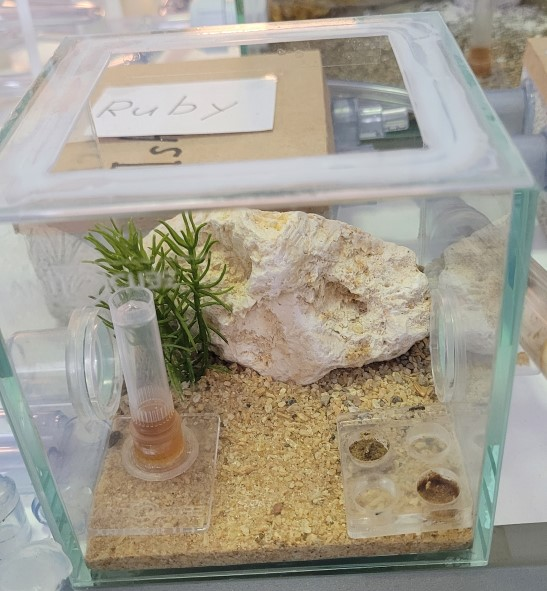
\includegraphics[width=.8\linewidth]{resources/F-rufibarbis.jpg}
    \caption[Waldameisen]{Waldameisen}
  \end{minipage}%
  \begin{minipage}{.5\textwidth}
  \end{minipage}
\end{figure}

\section{notwendig 2--3x die Woche}

\subsection{Zucker}\label{sec:Ameisen_sub:Zucker}
Zucker ist überlebensnotwendig für die erwachsenen Ameisen,
sonst haben sie nicht die Energie um in der Arena nach Futter zu suchen und die gesamte Kolonie kann sterben.

Daher bitte bei jeden Besuch überprüfen, ob die Zuckertränken noch voll sind oder sich Schimmel bildet.
Fällt der Füllstand in den geriffelten Bereich der Röhrchen\todo{Bild von Zuckertränke einfügen},
muss es wieder aufgefüllt werden\todo{Prozess beschreiben}.

Sollte ich Zuckerlösung in Reagenzgläsern angeschlossen haben\todo{Bild von Zuckerlösung in Reagenzglas},
besteht keine Gefahr, dass sie leergetrunken werden, jedoch setzen diese sehr schnell Schimmel an.
Ist das der Fall, bitte Zuckerlösung in Tränken in die Arena stellen und
wenn möglich das verschimmelte Reagenzglas entfernen und ausspülen\todo{beschreiben, wie Reagenzglas zu leeren ist}.

\subsection{Wasser}\label{sec:Ameisen_sub:Wasser}
Ameisen brauchen Zugang zu sauberem Wasser, daher bitte regelmäßig alle Wasserröhrchen\todo{Bild von Wasserröhrchen}
(eines pro Kolonie) kontrollieren:

\begin{itemize}
  \item\textit{Leichte Verfärbung des Wassers} \\
  kein Problem für 1--2 Wochen, wechseln kann warten bis ich zurück bin
  \item\textit{Starke Verfärbung des Wassers} \\
  wenn möglich bitte wechseln\todo{Prozess beschreiben}
  \item\textit{deutlicher Schimmel auf der Watte} \\
  bitte umgehend wechseln\todo{Prozess beschreiben}
  \item\textit{Erde auf der Watte} \\
  das ist normales Verhalten der Ameisen, kein Eingriff nötig
\end{itemize}

Tritt nichts davon auf, reichen die Röhrchen wochenlang, im Gut-Fall muss also gar nicht gewechselt werden.

\section{notwendig 1x die Woche}

\subsection{Nest befeuchten}\label{sec:Ameisen_sub:Befeuchten}
Die Nester der Wegameisen (mit der roten Folie) halten ihre Feuchtigkeit bis zu meiner Rückkehr,
nur das Nest der Waldameisen aus Luftbeton (mit der Abdeckung aus Pappe darauf) muss regelmäßig befeuchtet werden:
\begin{enumerate}
  \item Spritze mit stillem Mineralwasser füllen\todo{Bild on Spritze und Wasserflasche}
        (Leitungswasser kann Chlor enthalten, kann im Notfall aber auch verwendet werden)
  \item Papp-Deckel vorsichtig abnehmen (um die Bewohner nicht zu stören).\\
        Nicht erschrecken: darunter ist eine Glasscheibe, durch welche die Ameisen beobachtet werden können, aber sie können nicht heraus!
  \item Spritze in das Loch in der Scheibe einführen und langsam entleeren, bis Wasser aus dem Loch herauskommt.
  \item Spritze entfernen und ggf. überstehendes Wasser damit wieder aufsaugen
  \item Pappdeckel wieder aufsetzen
\end{enumerate}
Dieser Prozess darf gerne einmal zu Beginn des Besuchs durchgeführt und dann am Ende nochmal wiederholt werden,
wenn etwas Wasser in den Stein eingezogen und wieder Platz im Reservoir ist.

\subsection{Füttern}\label{sec:Ameisen_sub:Fuettern}
Ameisen brauchen Protein zum Wachsen, vor allem im Larvenstadium.
Erwachsene Ameisen brauchen kein Protein mehr, werden aber ihre Aktivität in der Arena
(und Ausbruchsversuche) verstärken, wenn nicht genug Protein da ist um die Jungen zu füttern.
Sollte mehrere Tage kein Protein zur Verfügung stehen, fangen Teile der Brut an zu sterben.
Ein paar Tage zu spät zu füttern stellt aber kein Problem dar, Ameisen legen Vorräte an.

\begin{itemize}
  \item Jede der Wegameisen Kolonien bekommt eine große Schabe\todo{Bild hinzufügen, wie Schaben aufzuschneiden sind}
        oder zwei bis drei Heimchen/Heuschrecken.
  \item Die Waldameisen bekommen eine kleine bis mittelgroße Schabe oder ein Heimchen.
        Diese Schalen sind dazu zu verwenden:\todo{Bild von Schalen hinzufügen}
\end{itemize}

\subsubsection{Alternative}
Wenn Schaben oder Heimchen nicht verfügbar sind, oder der Mut fehlt, kann Instant-Futter gegeben werden:
Für die Wegameisen eines der großen runden Schälchen etwa zur Hälfte mit Insektenpulver\todo{Bild von Puler} füllen\todo{bild von gefüllter Schule} und etwas Wasser einträufeln\todo{Bild von Spritze und Wasserflasche, Anzahl Tropfen angeben}.
Die Waldameisen bekommen zwei der kleinen Aussparungen im Vierertopf\todo{Bild vom gefüllten Vierertopf} auf dieselbe Weise gefüllt.
Es gibt zwei Arten von Insektenpulver im Kühlschrank, oberes Fach links, darf gerne abgewechselt werden. Sind diese leer finden sich weitere Röhrchen in Tüten im Tiefkühlfach, ebenfalls oberes Fach.

\section{Ausgebüchste Ameisen einfangen}
Wenn Ameisen entkommen sind, keine Panik! Sie \textit{wollen} wieder zurück ins Nest und entfernen sich nicht weit,
sie können einzeln mit einem Pinsel aufgetupft und wieder in die Arena gesetzt werden.
Größere Ausbrüche auf diese weise zu bekämpfen, kann zeitraubend sein.
Hinterher nach dem Loch suchen:
\begin{itemize}
  \item Ist ein Stöpsel herausgerutscht?
  \item Hat sich ein Schlauch gelöst oder ein Reagenzglas abgegangen?
  \item Ist eine der Schlauchkreuzungen aufgegangen? (Der Heißkleber hat sich ggf.\ abgelöst)
  \item Quetschen sie sich durch einen Spalt zwischen Arena und Deckel?
  \item Ist die weiße Barriere am Deckel an einer Stelle unterbrochen?
        (Hierfür muss man die Ameisen eine Weile bebachten um zu sehen, wo sie über die Barriere treten)
\end{itemize}
